% Do not change the section below
% ============================================================================
\documentclass[conference,compsoc,a4paper]{common/IEEEtran}
\IEEEoverridecommandlockouts
\usepackage{todonotes}
\usepackage{nimbusmononarrow}
\usepackage[T1]{fontenc}

\usepackage{balance}
\usepackage{cite}
\usepackage{amsmath,amssymb,amsfonts}
\usepackage{algorithmic}
\usepackage{graphicx}
\usepackage{textcomp}
\usepackage{xcolor}
\usepackage{subcaption}
\usepackage{url}
\usepackage{float}
\usepackage{hyperref} % https://tex.stackexchange.com/questions/151902/why-is-my-cross-reference-not-working-and-some-other-questions#:~:text=hyperref%20makes%20references%20click%2Dable%20hyper%20links%20(and%20has%20some%20more%20features).
\usepackage{dblfloatfix}
\usepackage{lipsum}

% This file contains configuration of the listings package, which is used to for the code
\usepackage{listings}
\usepackage{fontspec}
\usepackage{xcolor}

\lstdefinestyle{mystyle}{
    basicstyle=\fontsize{7.5}{10}\selectfont\ttfamily,
    captionpos=b,                    
}
\lstdefinestyle{mystyle1}{
    basicstyle=\fontsize{5.5}{10}\selectfont\ttfamily,
    captionpos=b,                    
}

% https://tex.stackexchange.com/a/377226
\definecolor{vgreen}{RGB}{104,180,104}
\definecolor{vblue}{RGB}{49,49,255}
\definecolor{vorange}{RGB}{255,143,102}
\definecolor{mygray}{RGB}{148,148,148}

\makeatletter
% \renewcommand*\verbatim@nolig@list{}
\newcommand*\@lbracket{[}
\newcommand*\@rbracket{]}
\newcommand*\@colon{:}
\newcommand*\colorIndex{%
    \edef\@temp{\the\lst@token}%
    \ifx\@temp\@lbracket \color{black}%
    \else\ifx\@temp\@rbracket \color{black}%
    \else\ifx\@temp\@colon \color{black}%
    \else \color{vorange}%
    \fi\fi\fi
}
\makeatother

\lstdefinestyle{verilog}
{
    language=Verilog,
    basicstyle=\fontsize{6}{8}\selectfont\ttfamily,
    keywordstyle=\color{vblue},
    identifierstyle=\color{black},
    commentstyle=\color{vgreen},
    numbers=left,
    numberstyle=\tiny\color{mygray},
    tabsize=4,
    breaklines=true,
    moredelim=*[s][\colorIndex]{[}{]},
    literate=*{:}{:}1,
    frame=single,
    % xrightmargin=1em,
    xleftmargin=1.5em, % https://tex.stackexchange.com/a/22372
    framexleftmargin=1.5em,
    numbersep=3pt
}

% Setting up the font
% https://tex.stackexchange.com/a/548156
\setmonofont{JetBrains Mono}[
    Contextuals = Alternate,
    Ligatures = TeX,
]
\lstset{
    basicstyle = \ttfamily,
    columns = flexible,
}

% https://tex.stackexchange.com/a/60870
\lstnewenvironment{code}[2][1]
{
    \lstset{
        language=verilog,
        style=verilog,
        numbers=left,
        caption=#2,
        firstnumber=#1 %https://tex.stackexchange.com/a/398628
    }
} {}

\newcommand{\codeword}[1]{\texttt{\footnotesize{#1}}}

\def\BibTeX{{\rm B\kern-.05em{\sc i\kern-.025em b}\kern-.08em
    T\kern-.1667em\lower.7ex\hbox{E}\kern-.125emX}}

\newcommand{\fixme}[1]{\textcolor{red}{[FIXME: #1]}}
% ============================================================================


% Add additional LaTeX packages if needed here
% ============================================================================
\usepackage[%
	detect-all,
	binary-units=true,
]{siunitx}
\usepackage{booktabs}
\usepackage{tikz}
\usepackage{common/moeptikz}
% ============================================================================


% Changing the look of the footnote
% https://tex.stackexchange.com/a/21917
\renewcommand{\footnoterule}{
	\kern -3pt
	\hrule width .4\columnwidth height 1pt
	\kern 2pt
}


\begin{document}

% Add paper title here; most likely you want to delete the \thanks{} macro
% ============================================================================
\title{HDL RISC-V-A Project Report}
% ============================================================================

% Update author information
% ============================================================================
\author{%
	\IEEEauthorblockN{%
		Nour Hadj Fredj, Mariia Kashirina, Roman Mishchuk, Mohamed Amine Jradi\\
		Prof. Dr. Carsten Trinitis\IEEEauthorrefmark{1}
	}
	\IEEEauthorblockA{%
		\IEEEauthorrefmark{1}Chair of Computer,       
            Information and Technology,
	}
	\textit{Department of Informatics}\\
	\textit{Technical University of Munich, Heilbronn, Germany}\\
	\textit{\textup\{nour.hadj-fredj, mariia.kashirina, roman.mishchuk, amine.jradi, carsten-trinitis\textup\}@tum.de}
}
% ============================================================================

\maketitle


% Edit include/abstract.tex to write your paper's abstract
% ============================================================================
%\begin{abstract}
%\input{include/abstract}
%\end{abstract}
% ============================================================================

% List keywords of your paper in lower-case below
% ============================================================================
% \begin{IEEEkeywords}
% RISC-V, ISA, Register, Register File, Address, ALU  
% \end{IEEEkeywords}
% ============================================================================

% For each section of your chapter, add one source file in the include folder
% ============================================================================
\section{Introduction}
In our project, we investigate how a 16-bit RISK-V architecture works.
We explore how simple arithmetic operations like multiplication and division are performed, their synthesis in combinatorial logic, and how other parts of the processor interact with each other.
We have done work to adjust the default structure of the RISK-V processor so that it matches the given specifications.
This report will give the reader a better understanding and an overview of RISK-V architecture.
The source code to the Verilog implementation of it and its test benches can be found online\footnote{At \url{https://github.com/superstudy160/HDL-RISC-V-i16-A-Project/}.}.

\subsection{Notation and terminology}

\begin{itemize}
    \setlength\itemsep{3pt}
    \item $R_i$ -- the $i$-th register of the processor;
    \item \codeword{MonoFont} -- the indication of a code snippet, parameter name of a keyword;
    \item \codeword{l} and \codeword{lv} -- parameters used throughout our code to specify the bitness of the parameters. By default, \codeword{l} = 16 (given that we are working with a 16-bit processor), and \codeword{lv} = 15 (the highest bit index of a 16-bit number). But we can decrease them for the testing purposes.
\end{itemize}
\section{Specifications}
We implemented a RISC-V module that consists of Instruction Memory, Control Unit, Register File (16-bit register length, 8 registers in total), and ALU. The usual Data Memory is removed, and results go back to the Register File, but the order and concrete Instructions themselves are hardcoded in the Instruction Memory module.

An Instruction is 16-bits long and can be understood in three different ways, depending on the operation we want to perform. Following Little Endian, bits [15:13] always stand for the opcode, and the next [12:10] bits represent the address of Register where the result of the operation will be stored. Then, for RRR-operation, bits [9:7] and [2:0] represent addresses of registers to fetch the data from. For RRI-operation, bits [9:7] are set for the register address, and the last [7:0] bits represent the immediate signed value. For LUI operation, we only need the resulting register and the immediate value to put to this register, so all [9:0] bits represent this value.

Program Counter is implemented and connected to the Instruction Memory where, depending on its value, it chooses a pre-coded instruction. The processor is able to perform multiplication (16-bit, RRR and RRI), division (16-bit, RRR and RRI), and load values to Registers. Everything is happening in a single cycle: the instruction is fetched from the Instruction Memory, the Control Unit receives an opcode and sends corresponding signals, ALU executes the instruction, and results come back to the Register File.

Processor implementation is also extended by creating a Flag Register which is not updated every Clock Cycle (Control Unit sends a special UpdateFlags signal if something needs to be written to Flag Register). 
\begin{table}[h] % Place the table here, or use other options like [htbp]
    \centering
    \caption{Flags Register reference}
    \label{tab:flags}
    \begin{tabular}{ccc} % Define the number of columns and their alignment
        \toprule % Top horizontal line
        index & Description  \\
        \midrule % Horizontal line
        0 & Multiplication overflow \\
        1 & Division has remainder \\
        2 & Division by zero \\
        3 & Division overflow ($-2^{(16-1)} \cdot -1$) \\
        \bottomrule % Bottom horizontal line
    \end{tabular}
\end{table}
\section{Instruction Memory}

The instruction Memory module stores the read-only instructions to be executed on the processor. The following subsections describe this module's design, implementation, and testing.

\subsection{Instruction Memory design}
\begin{figure}[H]
    \centering
    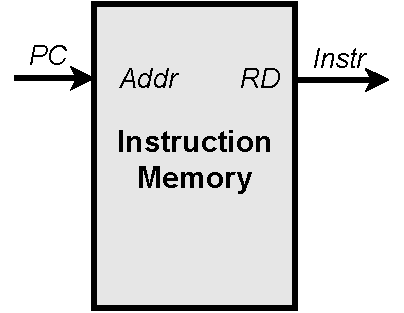
\includegraphics[width=.35\columnwidth]{pics/diagrams/riscv/modules/instruction_memory}
    \caption{Instruction Memory design}
    \label{fig:instruction_memory_module}
\end{figure}

\begin{itemize}
    \setlength\itemsep{3pt}
    \item \codeword{Addr} -- the address of the instruction to be read;
    \item \codeword{Instruction} -- the instruction read from the memory at the specified address.
\end{itemize}

\subsection{Instruction Memory implementation}

Since this memory is read-only, we hard-coded its contents in the module definition.

Data addressing is done byte-wise. Thus, given that instructions are 2 bytes long, we omit the first bit of the address when selecting the output (and so outputting the same instruction for both even and odd addresses).

We implemented such a behavior using the \codeword{case} statement:
\begin{code}[8]{Hard-coded Instruction example}
always @(Address) begin
case (Address[lv:1]) // Here we omit the first bit
    // This is the contents of the instruction memory
    00: Instruction = { 3'b011, 3'b000, 10'sd2 };
    ...
\end{code}

If the address goes out of the bounds of the memory, we return the default command, which does the multiplication of the $R_0$ by 1:
\begin{code}[17]{Default Instruction}
    ...
    default: Instruction = { 3'b001, 3'b000, 3'b000, 7'sd1 };
endcase
...
\end{code}


% \lstset{style=mystyle}
\section{Register File}
The Register File serves as a source for operands and a destination for storing results during arithmetic or logical operations. In instruction execution, the processor reads operands from the register file, performs operations, and writes results back to it.\newline
\subsection{Overview and Code implementation}
 We see that the Register File has as an input a clock signal, 3 addresses, InDataA, UpdateFlags and InNewFlags. For outputs we have We have OutDataB and C, OutFlags, and we also added a DebugData wire that we used to test our module and show the content of the registers. We have declared 3 Addresses for our input because our simplified RISC-V processor has 3 formats for instruction where RI type calls only one register, RRI type calls 2 registers and RRR types calls 3.\newline
\begin{figure}[H]
                \centering
                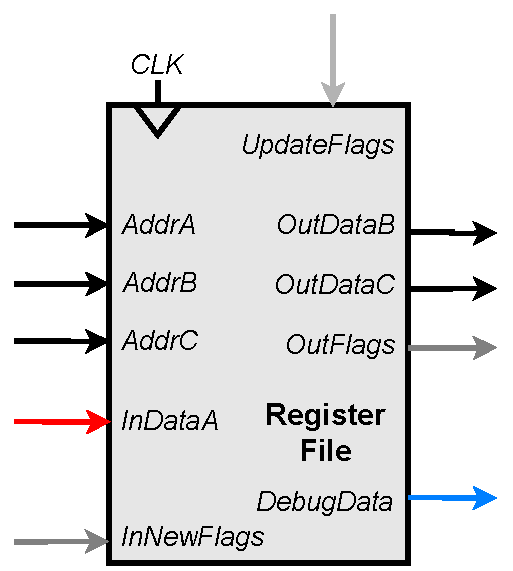
\includegraphics[width=.2\textwidth]{pics/diagrams/riscv/modules/register_file}
                \caption{Register file diagram}\
\end{figure}
After the input and output declaration, we specified that $R_7$ -- flags register using the following parameter:
\begin{code}[20]{Flags Register address}
	parameter FlagsAddress = 7;
\end{code}

Then we declared an array of registers named Data. This array consists of eight 16-bit registers which will be initialized to zero. \newline

This part is concerned with the read functionality of the Register File where we assign the data stored at the address specified by AddrB to OutDataB and we do the same for AddrC and OutDataC. We also assign the data stored in FlagsAddress to OutFlags. This allows us to read the content of the registers.\newline
\begin{code}[32]{Read functionality}
    assign OutDataB = Data[AddrB];
	assign OutDataC = Data[AddrC];
	assign OutFlags = Data[FlagsAddress[2:0]];
\end{code}
On the other hand, this section is responsible for the write functionality where on the positive edge of the clock signal, the block triggers and writes the input data InDataA into the register specified by AddrA. Also, if UpdateFlags is asserted, it updates the flags data stored at the address specified by FlagsAddress with the new flags data InNewFlags.\newline

\begin{code}[37]{Write functionality}
    always @ (posedge Clk) begin
		Data[AddrA] = InDataA;

		if (UpdateFlags)
		Data[FlagsAddress[2:0]] = InNewFlags;
	end
\end{code}
This final part has been added mainly for debugging and testing our Register File.\newline

Overall, our module implements a simplified register file with read and write functionality, flags update capability, and debug output for monitoring register content while operating synchronously with the clock signal.\newline
\section{Control Unit}

The control unit interprets instructions (opcodes) from the Instruction Memory and decodes them to determine what operations are to be performed. In the following subsections, we will discuss the Control Unit's behavior and how it is implemented.

\subsection{Behavior of Control Unit}

\begin{figure}[H]
    \centering
    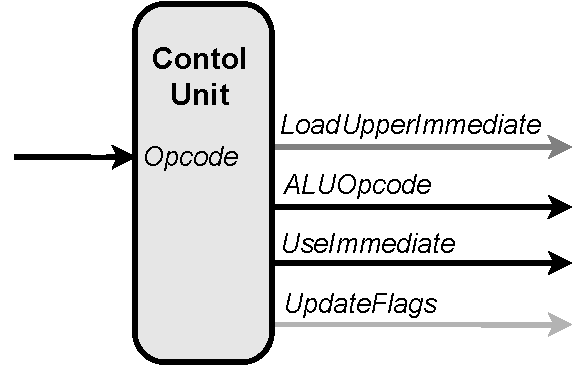
\includegraphics[width=.5\columnwidth]{pics/diagrams/riscv/modules/control_unit}
    \caption{Interface of the Control Unit}
    \label{fig:control_unit_module}
\end{figure}

When receiving an \codeword{Opcode}, the Control Unit outputs four different signals:
\begin{itemize}
    \setlength\itemsep{3pt}
    \item \codeword{LoadUpperImmediate}, which tells whether we need to store data from ALU or instruction (to execute LUI instruction);
    \item \codeword{ALUOpcode}, which sends ALU 0 or 1 depending on the type of operation we are performing (multiplication, division);
    \item \codeword{UseImmediate}, which tells whether the C operand is an immediate value or the value from the register file;
    \item \codeword{UpdateFlags}, which indicates whether the Register File should update flags after the operation or not.
\end{itemize}
    
An overview of the input and output signals of the Control Unit is shown in Figure \ref{fig:control_unit_module}.


\subsection{Implementation of Control Unit}

We have five different opcodes to be handled; they are 3 bits long and stored in [15:13] bits of the instruction. In the following, we will discuss the behavior of the Control Unit for each of these opcodes.


\textbf{Load Upper Immediate (LUI, 011)}

The dummy signal is sent to all inputs of ALU because there is no computation to do.

\begin{itemize}
    \setlength\itemsep{2pt}
    \item \codeword{ALUOpcode} = 0 (dummy signal);
    \item \codeword{UseImmediate} = 0 (dummy signal);
    \item \codeword{LoadUpperImmediate} = 1 -- in this case, we ignore ALU output and take the immediate value from the instruction;
    \item \codeword{UpdateFlags} = 0 -- there is no flags to update.
\end{itemize}

In all the following cases, the upper immediate value is ignored; thus, \codeword{LoadUpperImmediate} is set to 0.

\textbf{Multiplication (MUL, 111)}
\begin{itemize}
    \setlength\itemsep{2pt}
    \item \codeword{ALUOpcode} = 1 (multiplication);
    \item \codeword{UseImmediate} = 0 (RRR operation);
    \item \codeword{LoadUpperImmediate} = 0;
    \item \codeword{UpdateFlags} = 1 -- to renew the flags' state.
\end{itemize}

\textbf{Multiplication Immediate (MULi, 001)}
\begin{itemize}
    \setlength\itemsep{2pt}
    \item \codeword{ALUOpcode} = 1 (multiplication);
    \item \codeword{UseImmediate} = 1 (RRi operation);
    \item \codeword{LoadUpperImmediate} = 0;
    \item \codeword{UpdateFlags} = 1 -- to renew the flags' state.
\end{itemize}

\textbf{Division (DIV, 000)}
\begin{itemize}
    \setlength\itemsep{2pt}
    \item \codeword{ALUOpcode} = 0 (division);
    \item \codeword{UseImmediate} = 0 (RRR operation);
    \item \codeword{LoadUpperImmediate} = 0;
    \item \codeword{UpdateFlags} = 1 -- to renew the flags' state.
\end{itemize}
    
\textbf{Division Immediate (DIVi, 010)}
\begin{itemize}
    \setlength\itemsep{2pt}
    \item \codeword{ALUOpcode} = 0 (division);
    \item \codeword{UseImmediate} = 1 (RRi operation);
    \item \codeword{LoadUpperImmediate} = 0;
    \item \codeword{UpdateFlags} = 1 -- to renew the flags' state.
\end{itemize}

In the code, this logic is implemented using the case keyword:
\begin{code}[12]{Opcode switch-statement example}
    always @(Opcode) begin
	case (Opcode)
        // MUL
        3'b111: begin
            ALUOpcode = 1;
            UseImmediate = 0;
            LoadUpperImmediate = 0;
            UpdateFlags = 1;
        end
    ...
\end{code}

% \lstset{style=mystyle}
\section{ALU}
In the section we will focus on the ALU in the RISC-V architecture by explaining in detail how it works. The ALU is the arithmetic logic unit and in the context of this project, it will only do multiplication and division operations. 
\begin{figure}[H]
                \centering
                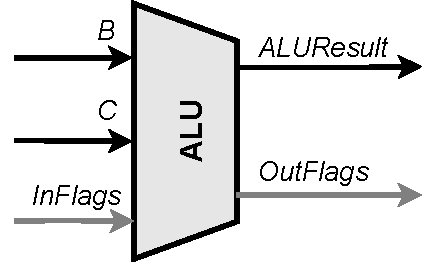
\includegraphics[width=.6\columnwidth]{pics/diagrams/riscv/modules/alu}
                \caption{ALU overview}\
\end{figure}
\subsection{Overview}
For an operation to be executed, the ALU receives a bit value from the control unit to indicate which operation to execute. As for the inputs, the ALU receives from the register file with the flags. For both operations, the ALU will first change the inputs to their absolute values.
\begin{code}{Assigning Absolute value operation}
wire [lv:0] AbsA;
AbsoluteValue #(l) abs_a(
	.A(A), .R(AbsA)
);
wire [lv:0] AbsB;
AbsoluteValue #(l) abs_b(
	.A(B), .R(AbsB)
);
\end{code}

According to the operation intended, the ALU will import the flags necessary. In case of multiplication, the ALU will update the value of multiplication overflow flag. 

\begin{code}{Assigning multiplication operation}
1: begin
    // Multiplication
    UnsignedR = MultiplicationR;
    FlagsOut[MultiplicationOverflowIdx[lv:0]] =
    MultiplicationOverflow | SignOverflow;
    FlagsOut[DivisionHasRemainderIdx[lv:0]] =                  FlagsIn[DivisionHasRemainderIdx[lv:0]];
    FlagsOut[DivisionByZeroIdx[lv:0]] =  FlagsIn[DivisionByZeroIdx[lv:0]];
    FlagsOut[DivisionOverflowIdx[lv:0]] = FlagsIn[DivisionOverflowIdx[lv:0]];
end
\end{code}

In our case when the operation wire has 1 then that indicates that a multiplication operation should be executed.
In the case of a division, there are two flags to be updated: divisionHasRemainder, which will indicate a remainder, and divisionDivByZero, which will indicate the edge case of division by zero. 

\begin{code}{Assigning division operation}
0: begin
// Division
UnsignedR = DivisionR;
FlagsOut[DivisionHasRemaindeFlagOut[lv:0]] = DivisionHasRemainder;
FlagsOut[DivisionByZeroFlagOut[lv:0]] = DivisionDivByZero;
FlagsOut[DivisionOverflowFlagOut[lv:0]] = SignOverflow;
FlagsOut[MultiplicationOverflowFlagOut[lv:0]] = FlagsIn[MultiplicationOverflowFlagOut[lv:0]];
end
\end{code}

In case of no flags are raised the noFlagsIdx. %not sure how it works
After doing the operation between two unsigned integers. The ALU operates to give a sign to the result.

\begin{code}{Sign operation}
reg [lv:0] UnsignedR;
wire SignOverflow;
GiveSign #(l) give_sign(
	.Sign(A[lv] ^ B[lv]),
	.A(UnsignedR),
	.R(R),
	.Overflow(SignOverflow)
);
\end{code}

The overall structure can be seen in Figure \ref{fig:alu_structure}:
\begin{figure}[H]
    \centering
    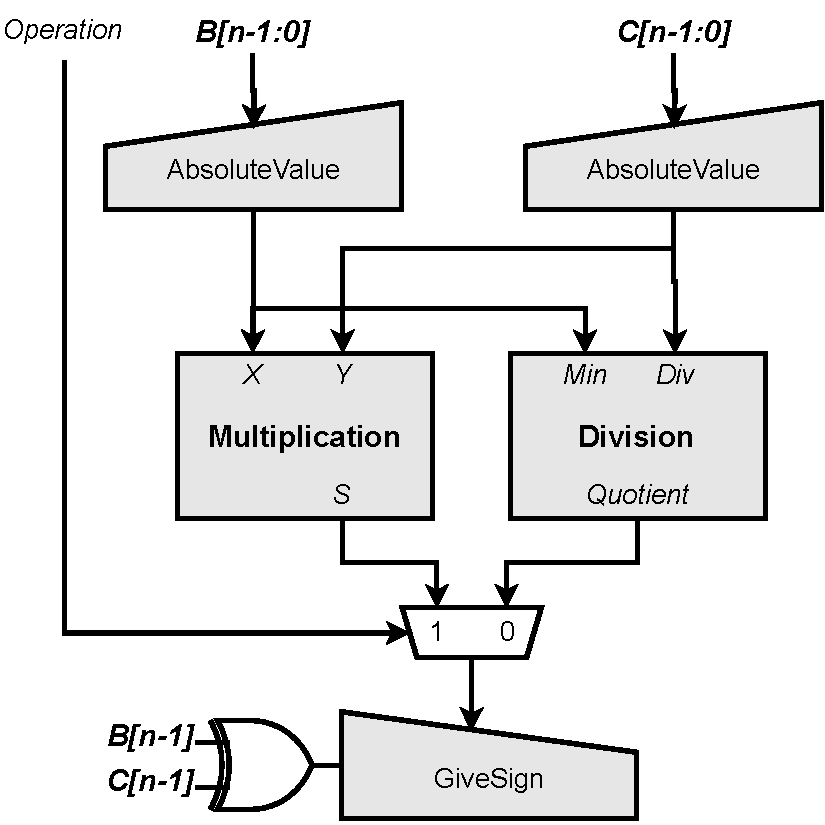
\includegraphics[width=.8\columnwidth]{pics/diagrams/riscv/modules/alu_structure}
    \caption{ALU structure}
    \label{fig:alu_structure}
\end{figure}

\subsection{Addition}
\begin{code}{1 bit adder}
module Adder (
	input X,
	input Y,
	input Cin,
	output S,
	output Cout
);

assign S = X ^ Y ^ Cin;
assign Cout = (X & Y) | ((X ^ Y) & Cin);

endmodule //Adder
\end{code}
We start by implementing one bit adder. Then we use it to implement a full adder for 16 bits.
\begin{code}[14]{Full adder }
module FullAdder #(parameter l = 16) (
	input [lv:0] X,
	input [lv:0] Y,
	input Cin,
	output [lv:0] S,
	output [lv:0] Cout
);

parameter lv = l-1;

wire [lv:0] Sum;
wire [l:0] Cout_temp;
assign Cout_temp[0] = Cin;

// Remaining bits
generate genvar i;
	for (i = 0; i <= lv; i = i + 1) begin
		Adder adder(X[i], Y[i], Cout_temp[i], Sum[i], Cout_temp[i+1]);
	end
endgenerate

assign S = Sum;
assign Cout[lv:0] = Cout_temp[l:1];

endmodule //FullAdder
\end{code}
We reimplement this full adder to make a full adder with overflow and carry flag. Overflow in case the addition of two positive number became negative because the range of bits representing the integers was exceeded. Carry in case the range of bits to represent the number was exceeded.
\begin{code}[49]{Full adder with flags}
module FullAdderFlags #(parameter l = 16) (
	input [lv:0] X,
	input [lv:0] Y,
	output [lv:0] S,
	output Overflow,
	output Carry
);

parameter lv = l-1;

wire [lv:0] Cout;

FullAdder #(l) full_adder (
	.X(X), .Y(Y), .Cin(1'b0),
	.S(S), .Cout(Cout)
);

assign Overflow = Cout[lv-1] ^ Cout[lv];
assign Carry = Cout[lv];

endmodule // FullAdderFlags
\end{code}
\subsection{Multiplication}
The multiplication is a composition of the addition operation and shift. That was the approach used, make the multiplication operation through the addition block we created.
In order for the multiplication to work we just copy the multiplier whenever we find a 1, then shift or skip and shift when we find a zero. We only add carries in the next operation for optimization purposes. So we do an addition operation then we add the result to the next addition operation and we add the carry too. That is the general concept. However, to optimize this operation, each time we shift we add the bits on the right to the final result and we keep going until the operation is finished. The result will be represented in 32 bit but we only compute the first 16 bits the second half is discarded and if it has some value in it then it is an overflow. These operations will be further explained one by one in the next sub-subsections.
Of course there are certain edge cases like carry and overflow which have specific flags to be raised when they happen.
\begin{figure}[H]
                \centering
                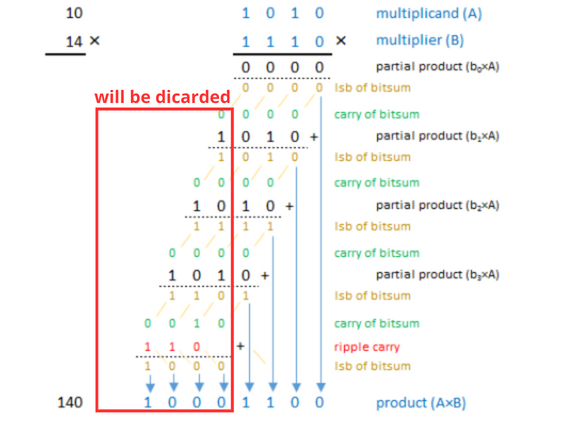
\includegraphics[width=.5\textwidth]{pics/multiplicationOp.png}
                \caption{Multiplication}\
\end{figure}
\subsubsection{Contolled adder circuit}
The controlled adder is the same as the 1 bit adder. As a matter of fact it uses the 1 bit adder we created only with one twist. we add another input to this controlled adder which is selection. This input will specify if we preceed with the addition or we ignore it and shift. In our case if the inpur is 1, we will preceed with the addition and if it is 0 we skip.\\
The figure below illustrate the diagram of controlled adder, as x, y, cin and selection are the inputs and cout and S are the outputs.
\begin{figure}[H]
                \centering
                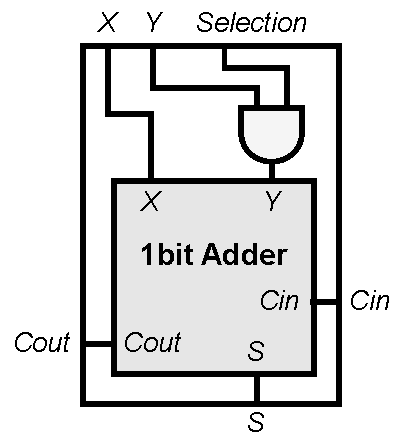
\includegraphics[width=.2\textwidth]{pics/diagrams/multiplication/controlled_adder.pdf}
                \caption{Controlled adder diagram}\
\end{figure}
\subsubsection{Contolled full adder circuit}
The controlled full adder circuit is the collection of the controller adder, which will allow us to do the same operation for 16 bits. So we just use the controlled adder multiple time. As for the carry we do not care about it as it will be passed to the next full adder. In other words cout for each controlled adder will not be connected to the next one rather to the one below it as shown in 3.3.3. This way we are multiplying one bit from the multiplier with all bits of the multiplicand.
\begin{figure}[H]
                \centering
                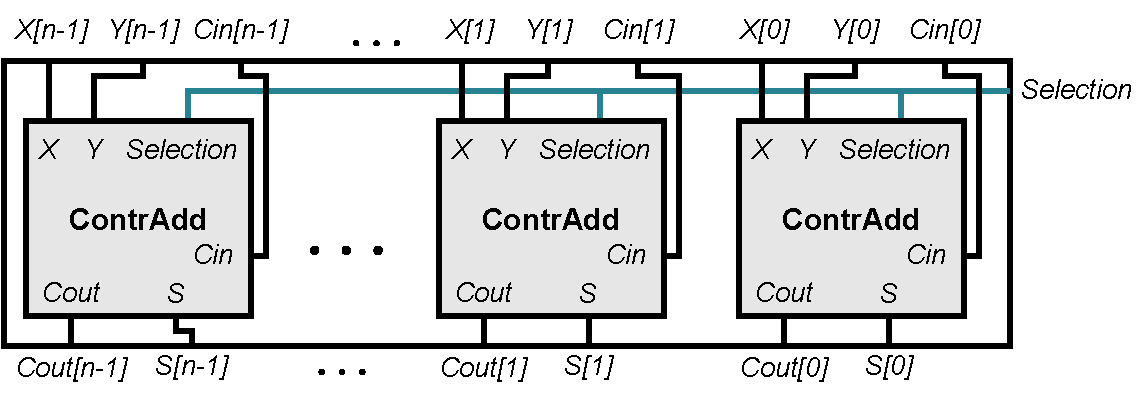
\includegraphics[width=.5\textwidth]{pics/diagrams/multiplication/controlled_full_adder.pdf}
                \caption{Controlled full adder diagram}\
\end{figure}
\subsubsection{Multiplication circuit}
Now we need to do the same operation of the controlled full adder 16 times.
This way we are multiplying each bit of the multiplier with all bits of the multiplicand. The result will be 32 bits. That is why we only compute the first 16 bits as we consider any bit out of that range overflow.\\
As shown in the simplified diagram below, if we are dealing with a 3 bit operation. The result will be 6 bits but we only compute the first 3 and we take the rest of the bits and the carry, we compare it with 0 to decide if there is a carry or an overflow.  
\begin{figure}[H]
                \centering
                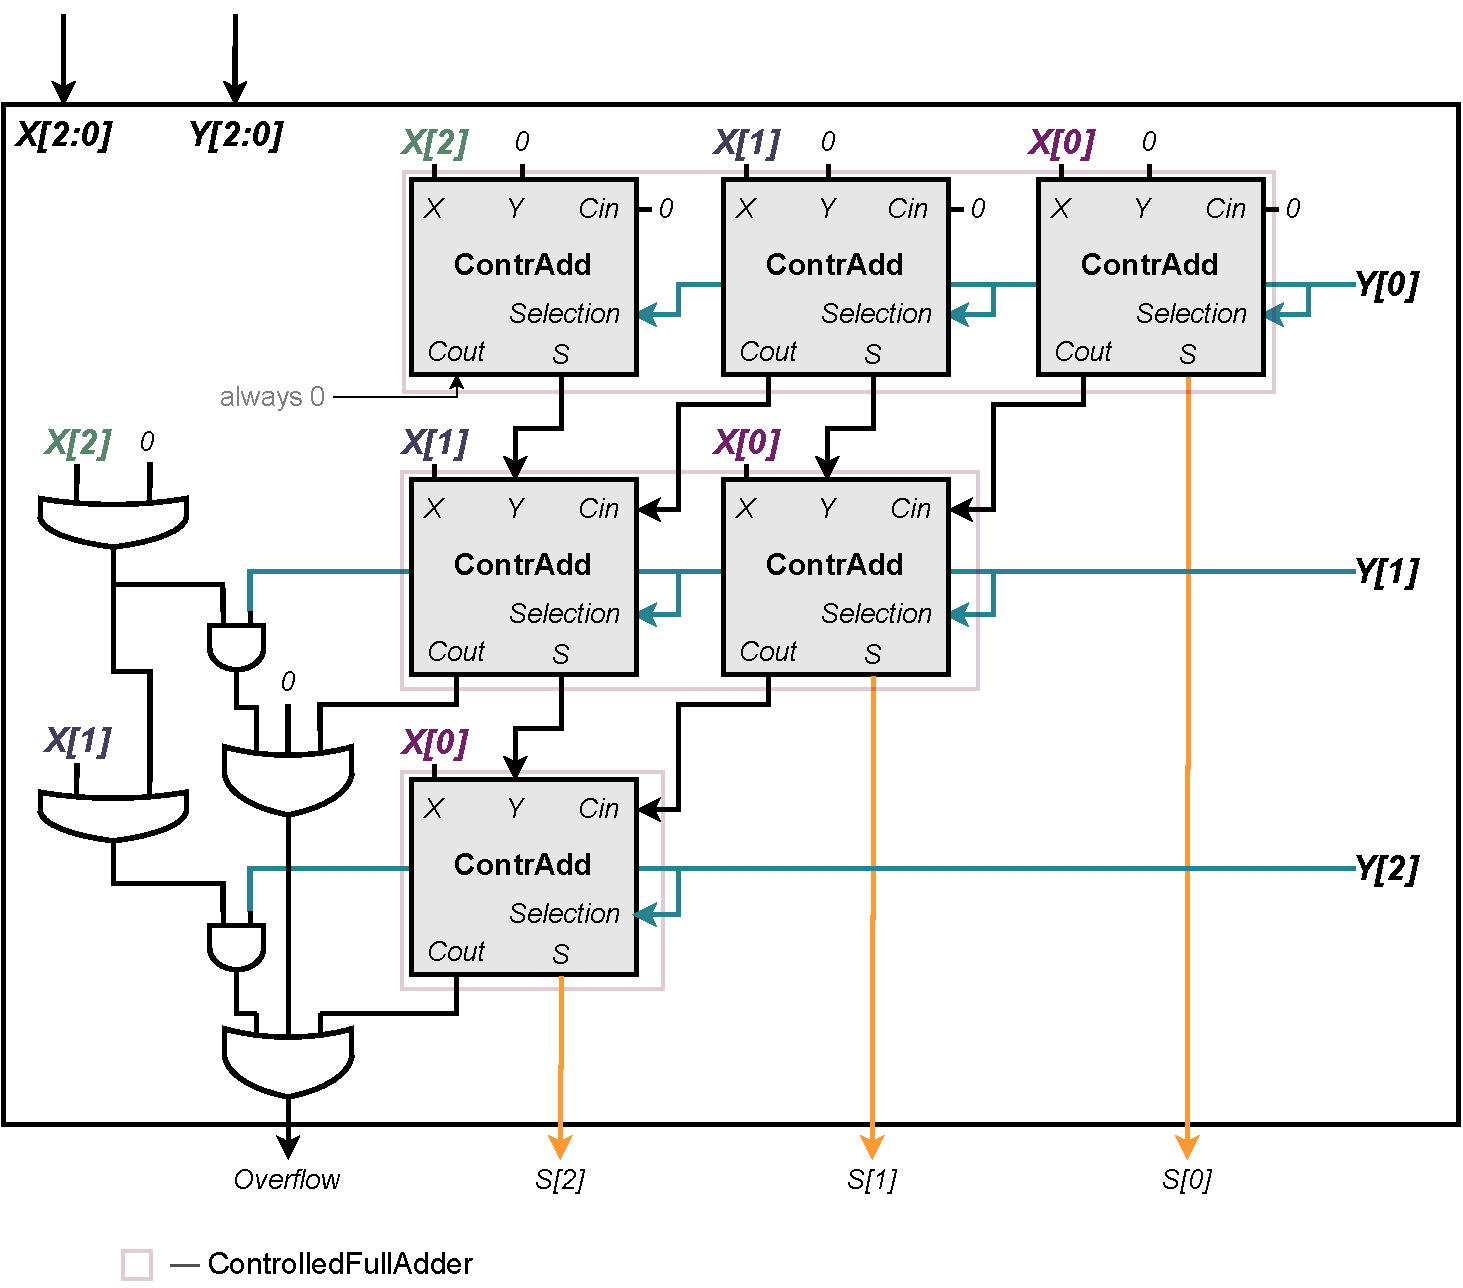
\includegraphics[width=.5\textwidth]{pics/diagrams/multiplication/multiplication.pdf}
                \caption{Multiplication diagram}
\end{figure}


\subsection{Division}
The division works similarly to the multiplication but with some changes. The division is a composition of the subtraction and shift operation.
That was the approach used, make the division operation through the subtraction block we created.
In order for the division to work we just copy the divider whenever we find a 0 in the borrow, then shift or skip and shift when we find a 1. So we do a subtraction operation then we shift and add the result to the next subtraction operation. That is the general concept. We created flags for division by zero and remainder. So for each case, a flag will be raised.
The division will be discussed in more detail in the next sub-subsections.
\begin{figure}[H]
                \centering
                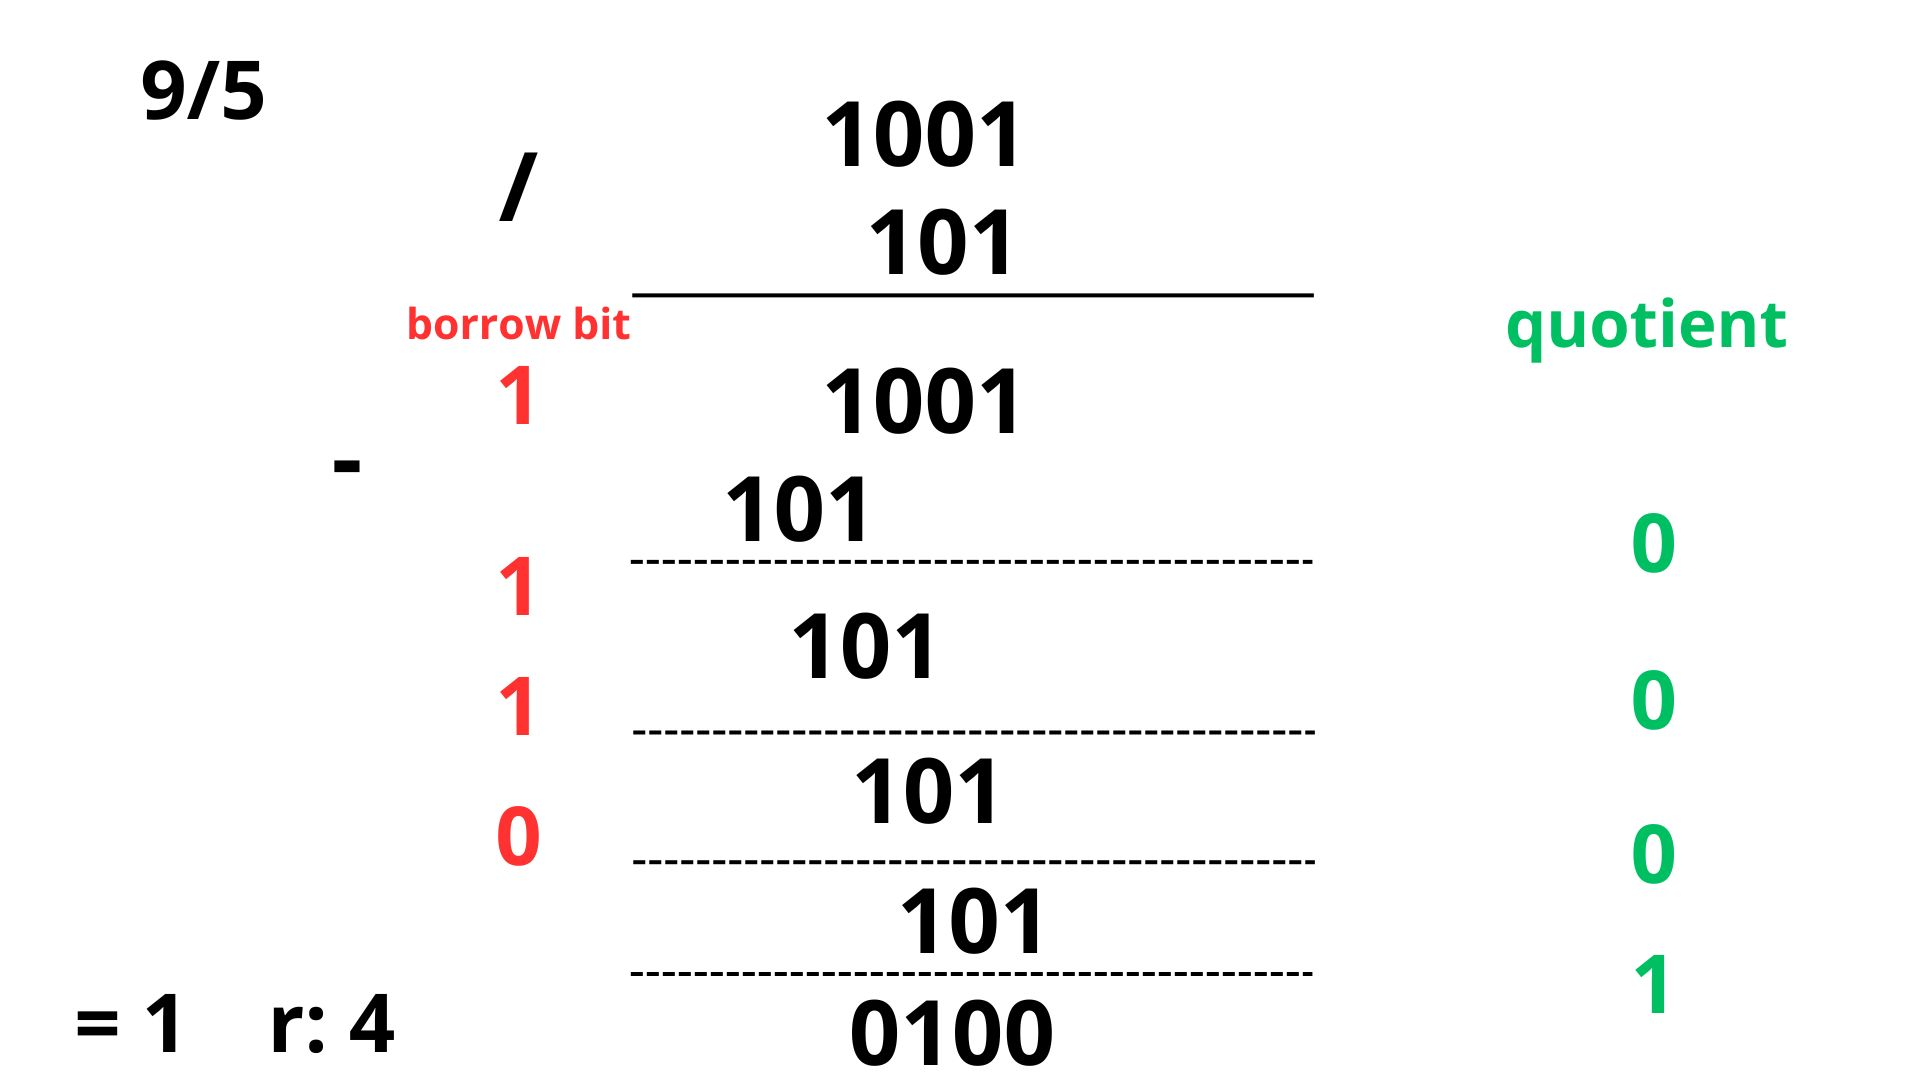
\includegraphics[width=.5\textwidth]{pics/devOp.jpg}
                \caption{Division}\
\end{figure}
\subsubsection{Subtractor}
This block is to subtract one bit from another.
To implement the subtraction we  use the following formulas:
\begin{align*}
D &= A \oplus B \oplus \text{Bin} \\
Bout &= (\neg A \land B) \lor ((\neg (A \oplus B)) \land \text{Bin})
\end{align*}
\subsubsection{Controlled subtractor}
The controlled subtractor, just like the controlled addition, is the same as a subtractor but with a small addition, which is the Selection input as shown in the diagram. Unlike the controlled addition, when the selection input is 0, the difference will be output as the difference. However when the selection is 1, the minuend will be out as the difference.
\begin{figure}[H]
                \centering
                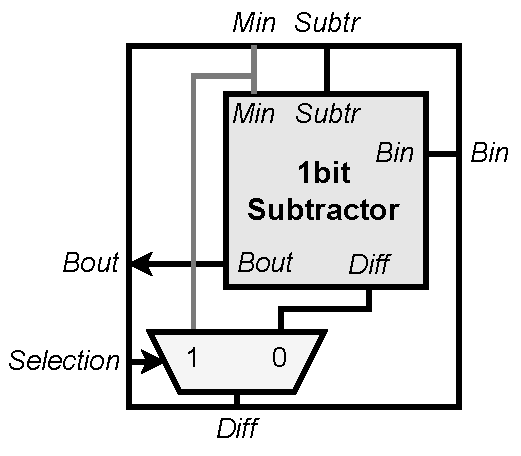
\includegraphics[width=.3\textwidth]{pics/diagrams/division/controlled_subtractor.pdf}
                \caption{Controlled subtractor diagram}\
\end{figure}
\subsubsection{Controlled full subtractor}
The controlled full substractor in the  collection of controlled subtractors. They are linked through the borrow out and borrow in as each borrow out becomes the borrow in of the next block. As shown in the figure, the output of the borrow out (Bout) will be forwarded to selection to determine if the output of the difference will be the difference or the minuend as explained in the previous sub-subsection. The Bout of the most significant bit is negated to form the quotient. If there is no borrow then the subtraction is possible and then the quotient bit in that block is 1 if not the the bit is 0. 
\begin{figure}[H]
                \centering
                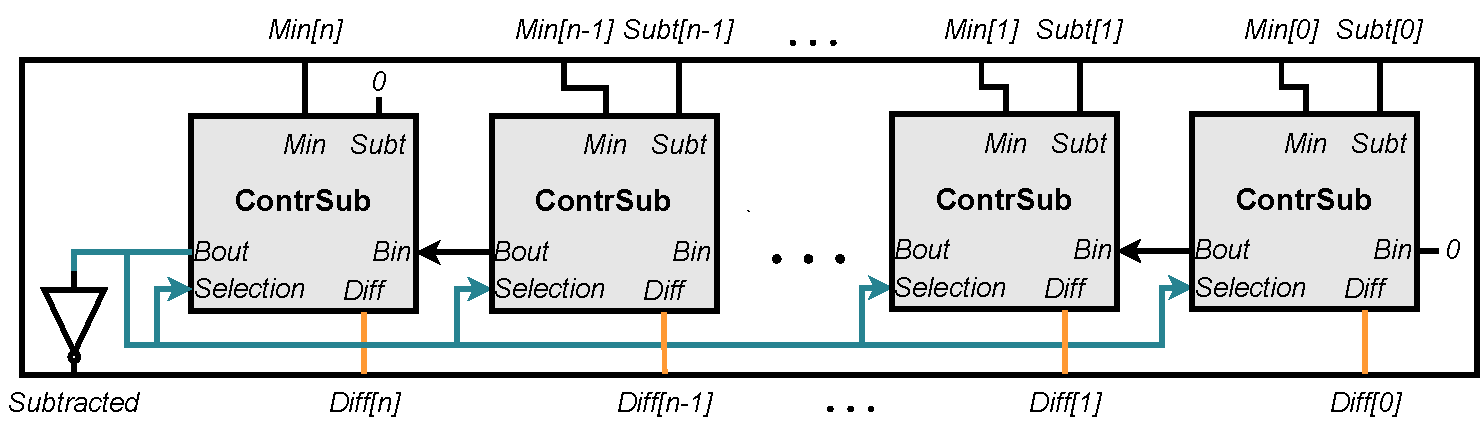
\includegraphics[width=.5\textwidth]{pics/diagrams/division/controlled_full_subtractor.pdf}
                \label{fig:controlled_full_subtractor}
                \caption{Controlled subtractor diagram}\
\end{figure}
\subsubsection{Division}
\begin{figure*}[!t]
    \centering
    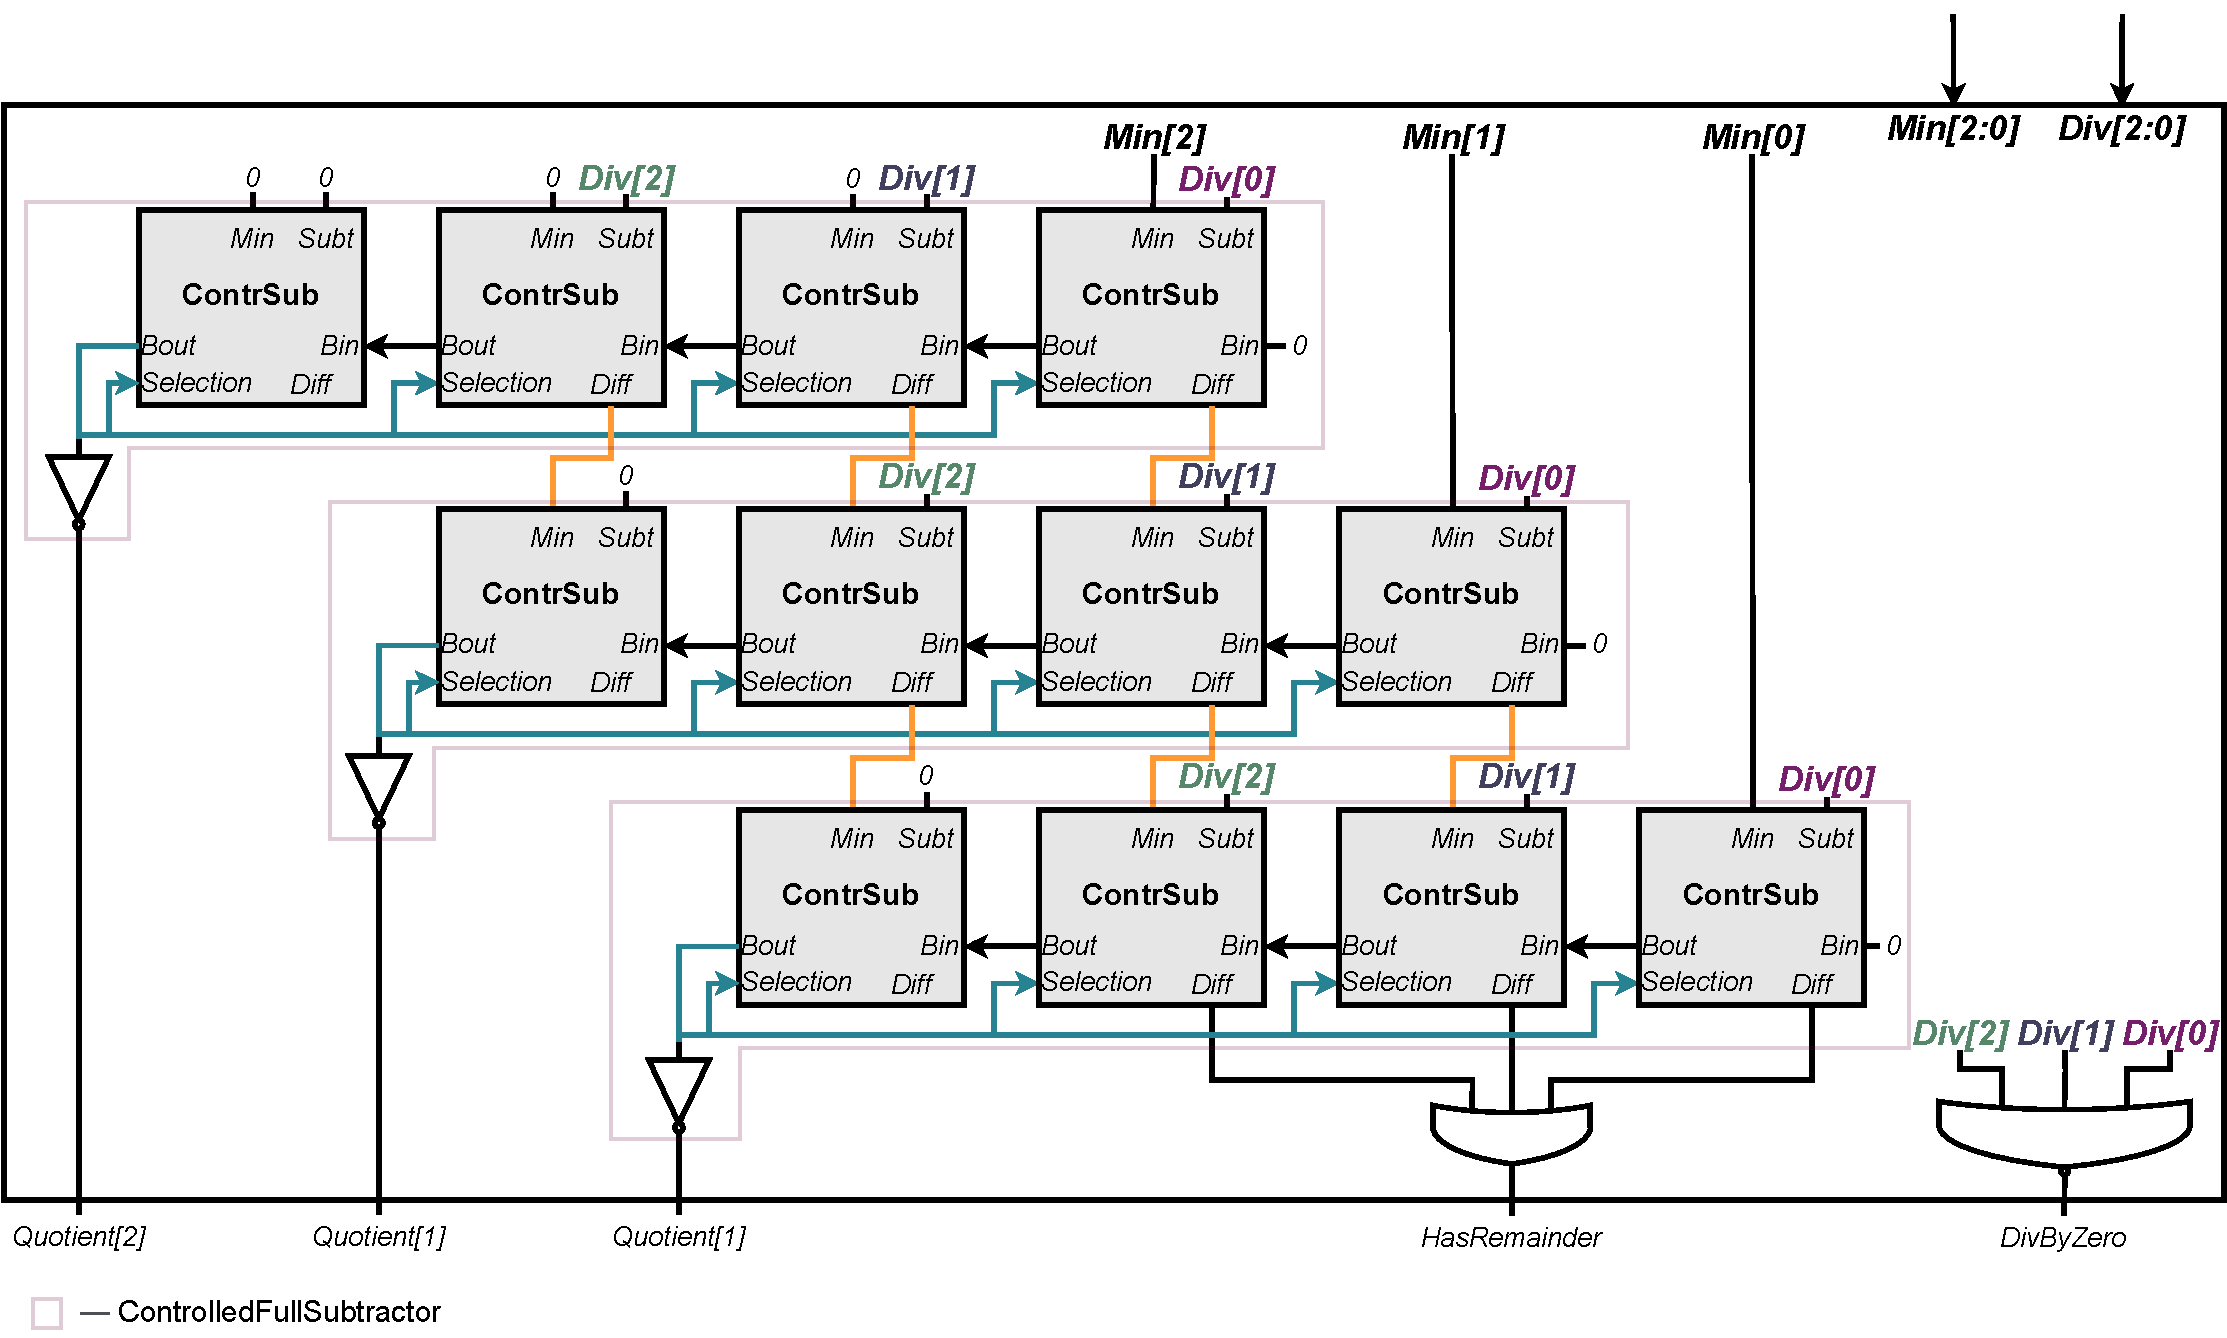
\includegraphics[width=.8\textwidth]{pics/diagrams/division/division}
    \caption{Division diagram}
    \label{fig:division}
\end{figure*}

Finally, to form the division operation, the combination of multiple layers of controlled full subtractor will result in the division operation. In the Figure \ref{fig:division} below, we can see a simplified division operation for two 3-bit integers. It is clear how the shift happens from layer to layer and within each layer, a bit from the minuend is included as input. the last block in the first layer is not an input block but rather a block so the most significant bit finds from where to borrow. The difference is forwarded from layer to layer bit by bit until it reached the end of the division where it will be forwarded to hasRemainder. If it is not 0 then the flag will be raised. Also if the divider is 0 it will also raise DivByzero. That is why we have NOR to check if we have a 000 or not.


\section{Debugging and testing}
\subsection{Instruction Memory test bench}

In the test bench, we iterated through all the memory addresses (including the out-of-bounds ones) and checked if the output was as expected:
\begin{code}[16]{}
initial begin
	$monitor("address=%d, instruction=%b\n", Address, Instruction);
	for (Address = 0; Address < 40; Address = Address + 1) begin
		#10;
	end
end
\end{code}
During the testing, we did not find any issues.
\subsection{Register File Test Bench}
This final part has been added mainly for debugging and testing our Register File.\newline

\begin{code}{Testing and Debugging}[47]
    generate
		genvar i;
		for (i = 0; i < r; i = i + 1) begin
		assign DebugData[i * l +: l] = Data[i[2:0]];
		end
	endgenerate
\end{code}

\subsection{Control Unit Test Bench}

In our implementation of the test bench, we went through all the possible opcodes and checked if the module output was correct.
\begin{code}[27]{Test Bench of Control Unit}
initial begin
    $monitor("LoadUpperImmediate=%d\nALUOpcode=%d\nUseImmediate=%d\nUpdateFlags=%d\n\n", LoadUpperImmediate, ALUOpcode, UseImmediate, UpdateFlags);
    
    $display("MUL:");
    Opcode = 3'b111;
    #10;
    ...
\end{code}
During the testing, we didn't find any issues.

\subsection{Addition Test Bench}
 In implementing the test bench, we went through all the possible edge cases, which are overflow, carry or overflow and carry at the same time.
 \begin{code}[20]{Addition Test Bench}
initial begin
	$monitor("  a=%b\n  b=%b\nsum=%b, o=%b, c=%b\n\n", a, b, sum, overflow, carry);
  ...
           
		x = 16'b1000000000110000;
		y = 16'b1000000011100000;
            #10;
  ...
		x = 16'b0111111111111111;
		y = 16'b0000000000000001;
		#10;
		x = 16'b1111111111111111;
		y = 16'b0000000000000001;
            #10;
	end
    ...
\end{code}
\subsection{Multiplication Test Bench}
In implementing the test bench, we went through all the possible edge cases, which is overflow. To make the overflow easier to detect we used in our test bench 3-bit integers.
 \begin{code}[23]{Multiplication Test Bench}
initial begin
...
		$monitor("X=%d,\nY=%d\nR1=%d, O=%b\n", X, Y, R1, Overflow);
  ...
		X = 16'd3;
		Y = 16'd4;
            #10;
    ...
\end{code}


\begin{figure*}[b]
	\centering
	\fbox{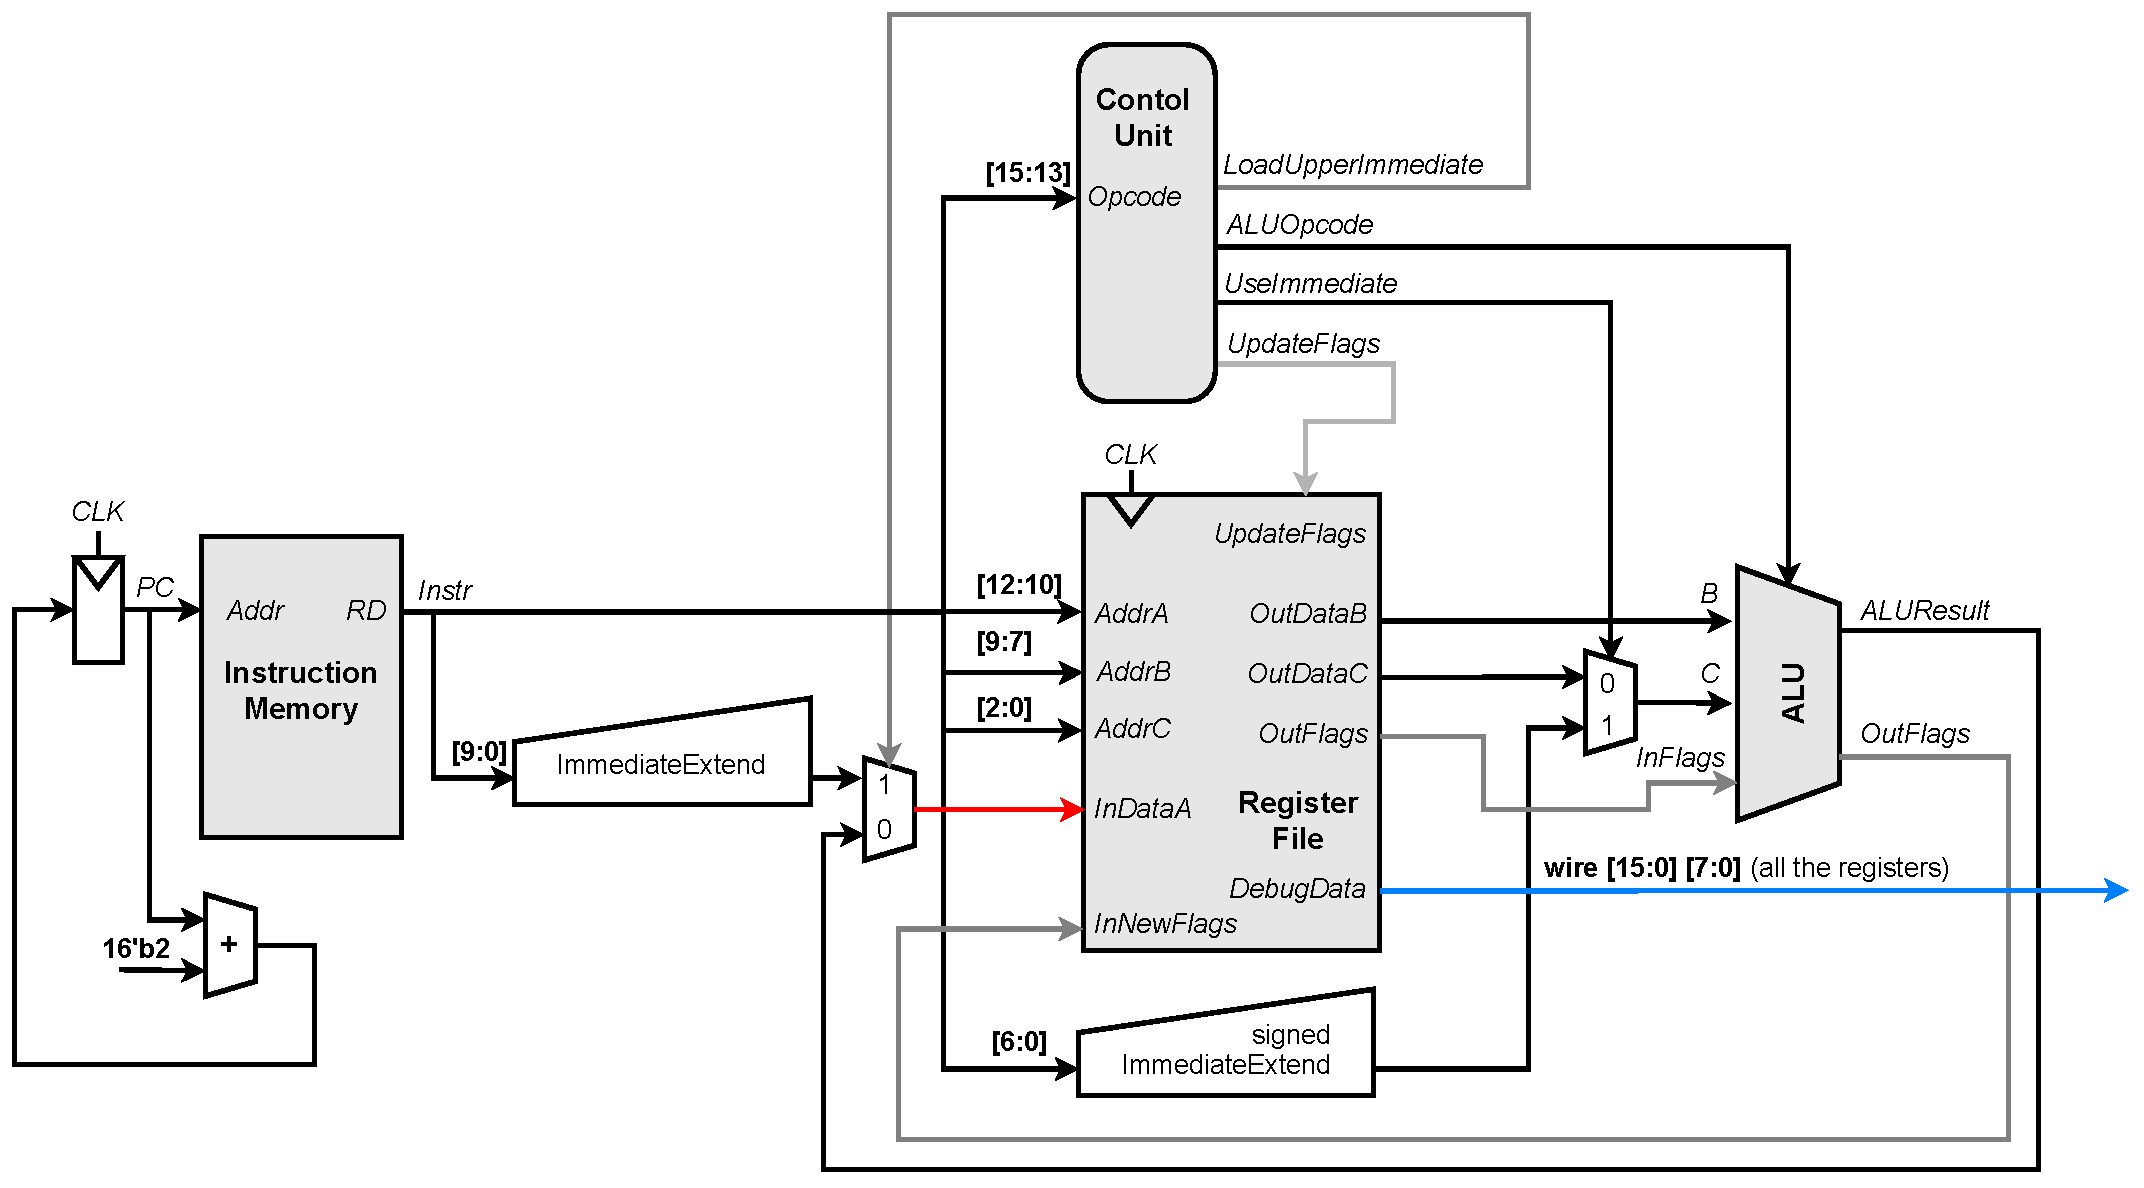
\includegraphics[width=.9\textwidth]{pics/diagrams/riscv/riscv.pdf}}
	\caption{Diagram of the RISC-V module.}
	\label{fig:riscv}
\end{figure*}

\subsection{Division Test Bench}
In implementing the test bench, we went through all the possible edge cases, which is divByzero and remainder. 
 \begin{code}[17]{Division Test Bench}
	initial begin
		$monitor("min=%d\ndiv=%d\nq=%d, r=%b, z=%b\n\n", min, div, quotient, HasRemainder, DivByZero);
		min = 16'd0;
		div = 16'd0;
		#10;
  ...
		min = 16'd7;
		div = 16'd0;
  	    #10;
		min = 16'd5;
		div = 16'd2;
            #10;
    ...
\end{code}
\subsection{ALU Test Bench}
In implementing the test bench, we went through all the possible edge cases of multiplication and division to make sure that all modules are connected and work correctly.
\section{RISC-V module}
We have explored how each module of the processor is implemented, and in this part of the report, we will show how they interact with each other. The design of the module is shown in Figure \ref{fig:riscv}.

\subsection{RISC-V execution flow}
Every new clock cycle, the Program Counter (PC) is increased by 2, which leads to the new Instruction being fetched from the Instruction memory.

Next, the bits [15:13] of the Instruction are loaded into the Control Unit as the Opcode. If the Opcode corresponds to LUI operation, then \codeword{LoadUpperImmediate} output would be set to 1 and \codeword{UpdateFlags} to 0. This would lead to the MUX controlling the Register File input, sending the data from ImmediateExtend, and the Register File not accepting the NewFlags from ALU.

Otherwise, the value sent to the Register File would result from ALU execution.

No flags are updated as the UpdateFlags signal was set to 0. If the Control Unit received the opcode that indicates an arithmetical operation, other bits of the Instruction will be understood as addresses of registers that the Register File will load to wires going to the ALU. If the OR gate receives the UseImmediate signal from the Control Unit, then instead of register C, the immediate value from signed ImmediateExtend will be put to the wire going to the ALU. Now, the ALU execution result is returned back to the Register File, and if no LoadUpperImmediate signal was received, the result goes to the Register, which address was specified in the Instruction. Also, with the result, New Flags are sent, and in case of an arithmetic operation, they are updated when the Register File receives the UpdateFlags signal. Finally, the new Clock cycle begins, the Program Counter is increased, and the whole cycle repeats again. 
\section{Conclusion}
In conclusion, our project involved customizing the RISC-V architecture to achieve our specific goals, enabling the successful implementation of register loading, multiplication, and division using combinational logic. While we have made significant progress in understanding and implementing the hardware aspects of these operations, there is still potential for further optimization to improve their speed. It's important to note that optimizing the propagation time of multiplication and division may result in an increased number of gates. Finding a balance between faster operations and efficient use of hardware resources is crucial. Our project represents an initial exploration into hardware-level operations.
% ============================================================================


% Put your references in the paper.bib file
% ============================================================================
\nocite{*}
\balance
\bibliographystyle{IEEEtran}
\bibliography{paper}
% ============================================================================
\end{document}
